\documentclass[../main.tex]{subfiles}

\begin{document}

A basic goal of every communication network is to handle the traffic injected by its nodes by limiting the rate of transactions joining the network. In fact, such a traffic could lead to unpleasant situations such as network congestion, due to resource limitations, or spam, due to malicious actors:

\begin{itemize}
    \item \textit{Congestion control.} In most networks, there are circumstances where the incoming traffic load is larger than what the network can handle. If nothing is done to restrict the influx of traffic, bottlenecks can slow down the entire network. A similar analysis can be applied to distributed ledgers, where the incoming traffic (i.e., transactions issued by the nodes of the network) exploits limited resources such as bandwidth, computational power, or disk space. Additionally, nodes can lose synchronization with each other, sometimes without being aware of it.
    \item \textit{Spam detection.} Gossip protocols (which are currently implemented to forward transactions in the IOTA network) are an efficient and reliable way to disseminate information. These protocols have nevertheless a drawback: They are unable to limit the dissemination of spam messages. Indeed, messages are redundantly distributed in the network and it is enough that a small subset of nodes forward spam messages to have them received by a majority of nodes.
\end{itemize}

Rate limitation strategies for communication networks are well studied in the case of both congestion control~\cite{kelly1998} and spam detection~\cite{dwork1993}. The former has been deeply investigated after the Internet collapse in the 80's, and solutions based on \textit{Additive Increase Multiplicative Decrease} have been proposed to properly modulate the influx of packets in the network~\cite{corless2016aimd, chiu1989, jacobson1988}. We plan to adopt a similar strategy to deal with potential congestion in the Tangle. On the other hand, the seminal work by Dwork and Naor~\cite{dwork1993} in 1993 paved the way to research in spam prevention. In the context of DLTs, many blockchains use PoW as a built-in rate limitation mechanism. However, PoW leads to undesirable side effects such as mining races: The discrepancy between smaller general purpose devices and optimized hardware with respect to the PoW performance is several orders of magnitude. Hence, any rate control based on PoW would eventually leave smaller devices behind. A new transaction rate control mechanism for the Tangle is therefore required to deal with the global and per-node limitations of the network. In the rest of the section, we will investigate two anti spam mechanisms based on varying difficulty PoW (Section~\ref{sec:adaptive_pow}) and on non-parallelizable functions (Section~\ref{sec:vdf}).

\subsection{Adaptive PoW}\label{sec:adaptive_pow}

In a pure PoW-based architecture, a high difficulty value would prevent low-power nodes from issuing transactions, which is not desirable, especially in the context of Internet-of-Things; on the other hand, low difficulty can quickly lead to network congestion. We propose an adaptive PoW algorithm to allow every node to issue transactions while penalizing spamming actions.

\subsubsection{Algorithm}

All nodes in the network have knowledge of three global parameters:

\begin{itemize}
    \item \textit{Base difficulty} $d_0$. It sets the minimum difficulty of PoW.
    \item \textit{Adaptation rate} $\gamma_i\in [0, 1]$. It provides the rate at which the PoW difficulty will be adjusted, which depends on the mana $m_i$ owned by node $i$.
    \item \textit{Time window} $W>0$. This parameter defines the granularity of the algorithm, and its role will be clarified below.
\end{itemize}

Similarly to the current implementation, issuing a new transaction must be preceded by the computation of some PoW. At time $t$, node $i$ must perform a PoW with difficulty $d_i(t)$ which can be calculated by
\begin{equation}\label{eq:difficulty}
    d_i(t) = d_0 + \left \lfloor{\gamma_i\cdot a_i(t)}\right \rfloor,
\end{equation}
where $a_i(t)$ represents the number of transactions issued by node $i$ in the time interval $[t-W, t]$. Note that when $\gamma_i=0$, the algorithm becomes equivalent to the current IOTA implementation.

Again, received transactions are processed in FIFO order. Let us assume we receive a transaction with difficulty $d_i$ signed by node $i$. To decide whether this transaction should be forwarded or not, a node counts how many transactions $r_i(t)$ signed by $i$ has been received in the last $W$ seconds. In accordance to the formula given by Eq.~\eqref{eq:difficulty}, the node forwards the transaction if the following condition is satisfied:
\begin{equation*}
    d_i\geq d_0 + \left\lfloor{\gamma_i\cdot r_i(t)}\right\rfloor.
\end{equation*}

Due to the asynchronous nature of the system, some of the transactions may be received in burst, invalidating the previous formula. We consider a correcting term $c>0$ which allows to accept transactions with lower difficulty. This parameter is known by all nodes. We modify the previous formula into:

\begin{equation*}
    d_i\geq \max\{d_0; \ d_0 + \left\lfloor{\gamma_i\cdot r_i(t) - c}\right\rfloor\}.
\end{equation*}

For the sake of simplicity, we assume incoming transactions are checked in the same order as they are issued by the sending node.
As the expected time needed to perform the PoW is typically much larger than the network latency $h$, this is a reasonable assumption.

Assume that a transaction is seen for the first time at time $t_0$. Every node will store the $id$ of the node issuing the transaction, the PoW difficulty computed and the time $t_0$. The identity $id$ of the issuing node as well as its mana $m_{id}$ can be determined using the methods described in Section~\ref{sec:node_acc}. Based on this information, it can then be checked that the difficulty of the most recent transaction is indeed sufficient.
This idea is more formally described in Algorithm~\ref{alg:rate_control}.

\begin{algorithm}[htb]
\SetKwFunction{time}{time}\SetKwFunction{node}{nodeId}\SetKwFunction{difficulty}{difficulty}
\KwIn{incoming transaction $tx$, set of known transactions $\mathcal{X}$, time window $W$, basic difficulty $d_0$, adaptation rate $\gamma_i$.}
\KwOut{forward or ignore $tx$.}
\BlankLine 
$t_0$ $\gets$ \time{tx}\;
$id$ $\gets$ \node{tx}\;
$\mathcal{T}$ $\gets$ $tx'\in\mathcal{X} \ | \ \time{$tx'$} \in \left(t_0-W,t_0\right] \wedge \node{tx'} = id$\;
\BlankLine
\If{$\difficulty{tx} \geq d_0 + \gamma_i\cdot |\mathcal{T}|$ }{
\Return forward $tx$\;
}
\Return discard $tx$\;
\caption{Rate control algorithm}
\label{alg:rate_control}
\end{algorithm}

\subsubsection{Theoretical analysis}

In the IOTA protocol implementation the number of operations triples for each increment of the difficulty. Let $b$ be the \textit{mean} number of operations needed to solve the PoW at difficulty $1$. Furthermore, following the definition of $gamma$, $1/\gamma$ is the maximum number of transactions that can be sent at a given difficulty during a time window $W$ (note that we omit the index $i$ as we perform the analysis on a single node). Hence, the number of operations that can be computed by a node during a time window, i.e., $\mu\cdot W$, produces a bound on the node's throughput:
    \begin{align*}
        \mu\cdot W &\geq \frac{b\cdot 3^{d_0}}{\gamma} + \frac{b\cdot 3^{d_0+1}}{\gamma} + \ldots + \frac{b\cdot 3^{d_0+n}}{\gamma}\\
        &= \frac{b}{\gamma}\cdot\sum_{i=0}^n3^{d_0+i}\\
        &= \frac{b}{\gamma}\cdot\frac{3^{d_0+n}-1}{3^{d_0}-1},
    \end{align*}
    which, after elementary computations, gives
    \begin{align}\label{eq:n-bound}
        n &\leq\log_3\left(\frac{\gamma\cdot W\cdot(3^{d_0}-1)}{b}\cdot\mu+1\right) - d_0\nonumber\\
        &\approx \log_3\left(\frac{\gamma\cdot W}{b}\cdot\mu\right).
    \end{align}
    Furthermore, consider that the throughput is equal to the total number of transactions issued by a node, i.e., $\frac{n-d_0}{\gamma}$, over a time window $W$. Hence, the throughput for a node with computational capability $\mu$ is
    \begin{align*}
        \theta(\mu)&=\frac{n-d_0}{\gamma\cdot W}\\
        &\leq \frac{\log_3\left(\frac{\gamma\cdot W}{b}\cdot\mu\right) - d_0}{\gamma\cdot W}.    \end{align*}


\subsubsection{Simulations}

We built a Python simulator with Jupyter notebook\footnote{\url{https://github.com/iotaledger/adaptive-pow-sim}} in order to verify whether the adaptive PoW algorithm can mitigate the problems described in the beginning of this section. In the simulations, we considered a simple scenario with a single node to evaluate the maximum throughput it can generate.

Suppose a node has computational capability $\mu$ measured in number of operations per second. We assume a node can belong to one of the following three categories depending on its computational power:
\begin{itemize}
    \item IoT, where $\mu = 10^{-1}\times 10^6$;
    \item Laptop, where $\mu = 10^{0}\times 10^6$;
    \item FPGA, where $\mu = 10^{6}\times 10^6$.
\end{itemize}

Furthermore, we assume that the number of operations needed to solve PoW at difficulty 14 is a random variable uniformly distributed with mean $3^{14}~\approx~5\times 10^{6}$. Hence, an IoT device will be able to solve it with an average time of 1 minute.

Finally, we set the following global parameters:
\begin{itemize}
    \item Base difficulty $d_0 = 10$;
    \item Adaptation rate $\gamma = 0.1$, which means the node increases the PoW difficulty every 10 transactions sent within the time window;
    \item Time window $W = 1000$ s.
\end{itemize}
 
In the following subsection, we present the simulation results when a node wants to issue 5000 transactions in the shortest possible time, i.e., we aim to maximize the total throughput.

In this subsection, we present the simulations results based on the current fixed PoW algorithm, i.e., when $\gamma = 0$. In Fig.~\ref{fig:time_fixed}, we show the time (in seconds) needed to compute the PoW for IoT, laptop and FPGA. The red line shows the average time needed to compute the PoW. As we expect, IoT devices require on average 1 minute for a PoW difficulty of 14. Laptops improve this time to about 6 seconds, while FPGAs run 6 orders of magnitude faster than laptops (i.e., they solve the PoW in a few microseconds).

According to these numbers, in Fig.~\ref{fig:tps_fixed} we show the throughput generated by the nodes, computed as the number of transactions per second. In the current IOTA implementation, the usage of FPGAs can speed up the computation by several orders of magnitude, preventing low-power nodes to access the network successfully and enabling spam attacks.

\begin{figure*}
    \centering
    \begin{subfigure}[b]{\textwidth}
        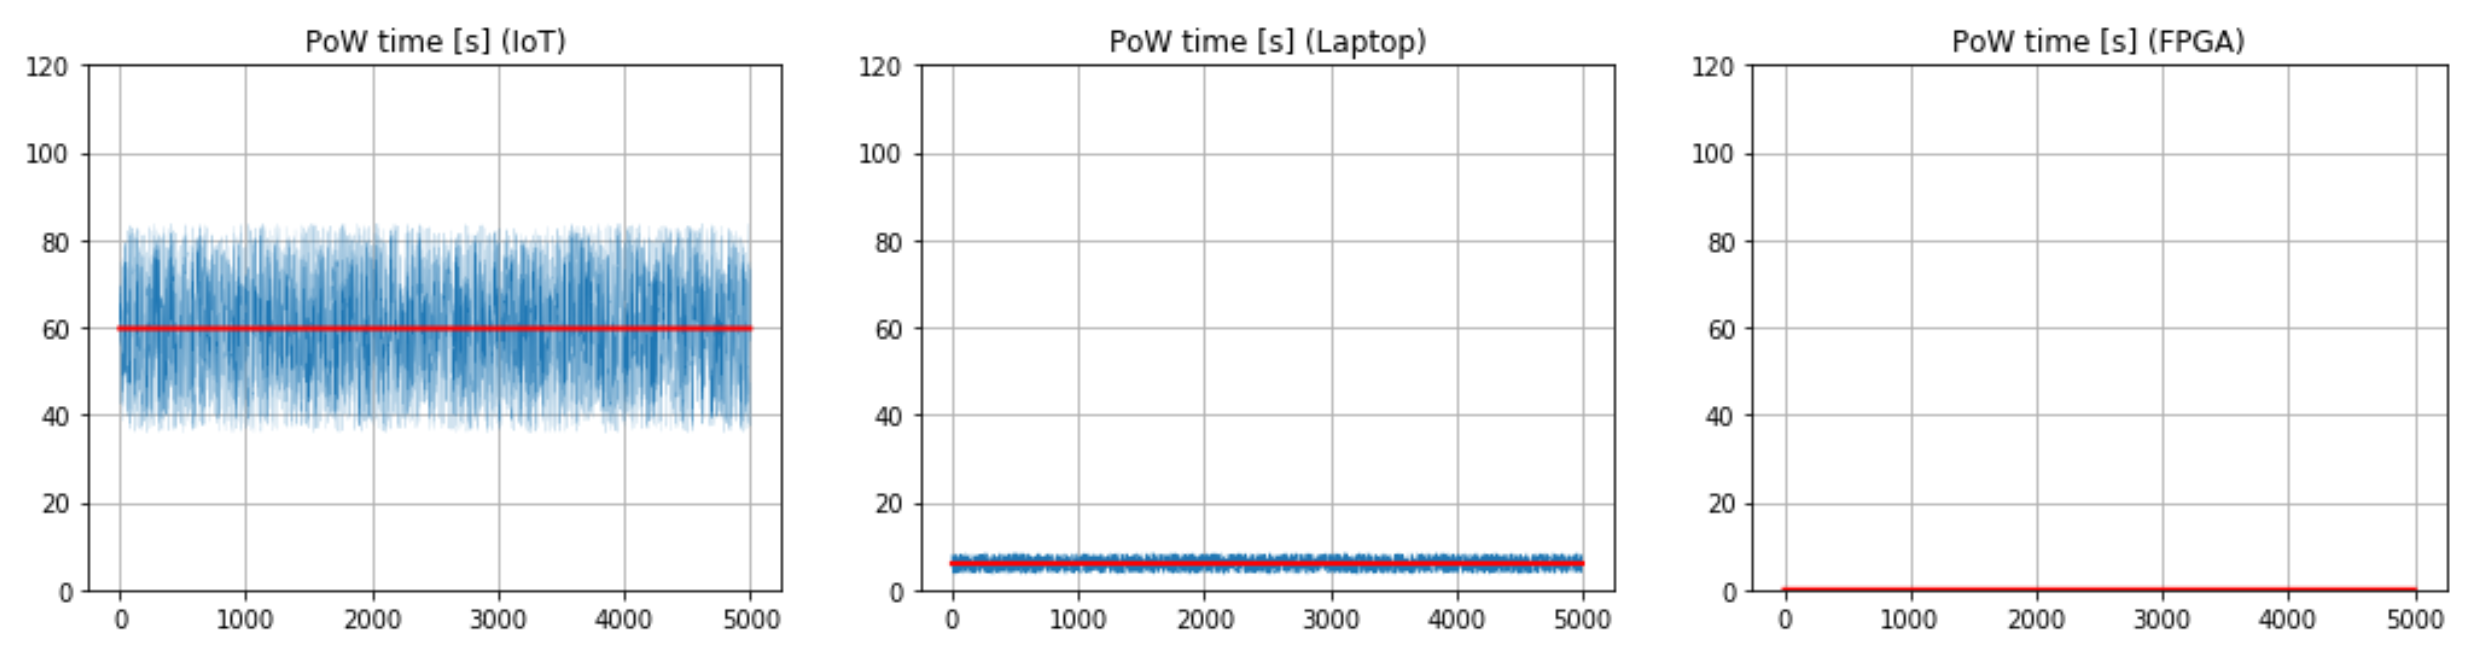
\includegraphics[width=\linewidth]{images/time_fixed.PNG}
        \caption{Time (in seconds) needed to compute fixed PoW (difficulty = $14$). The red line shows the average PoW time.}
        \label{fig:time_fixed}
    \end{subfigure}
    
    \begin{subfigure}[b]{\textwidth}
        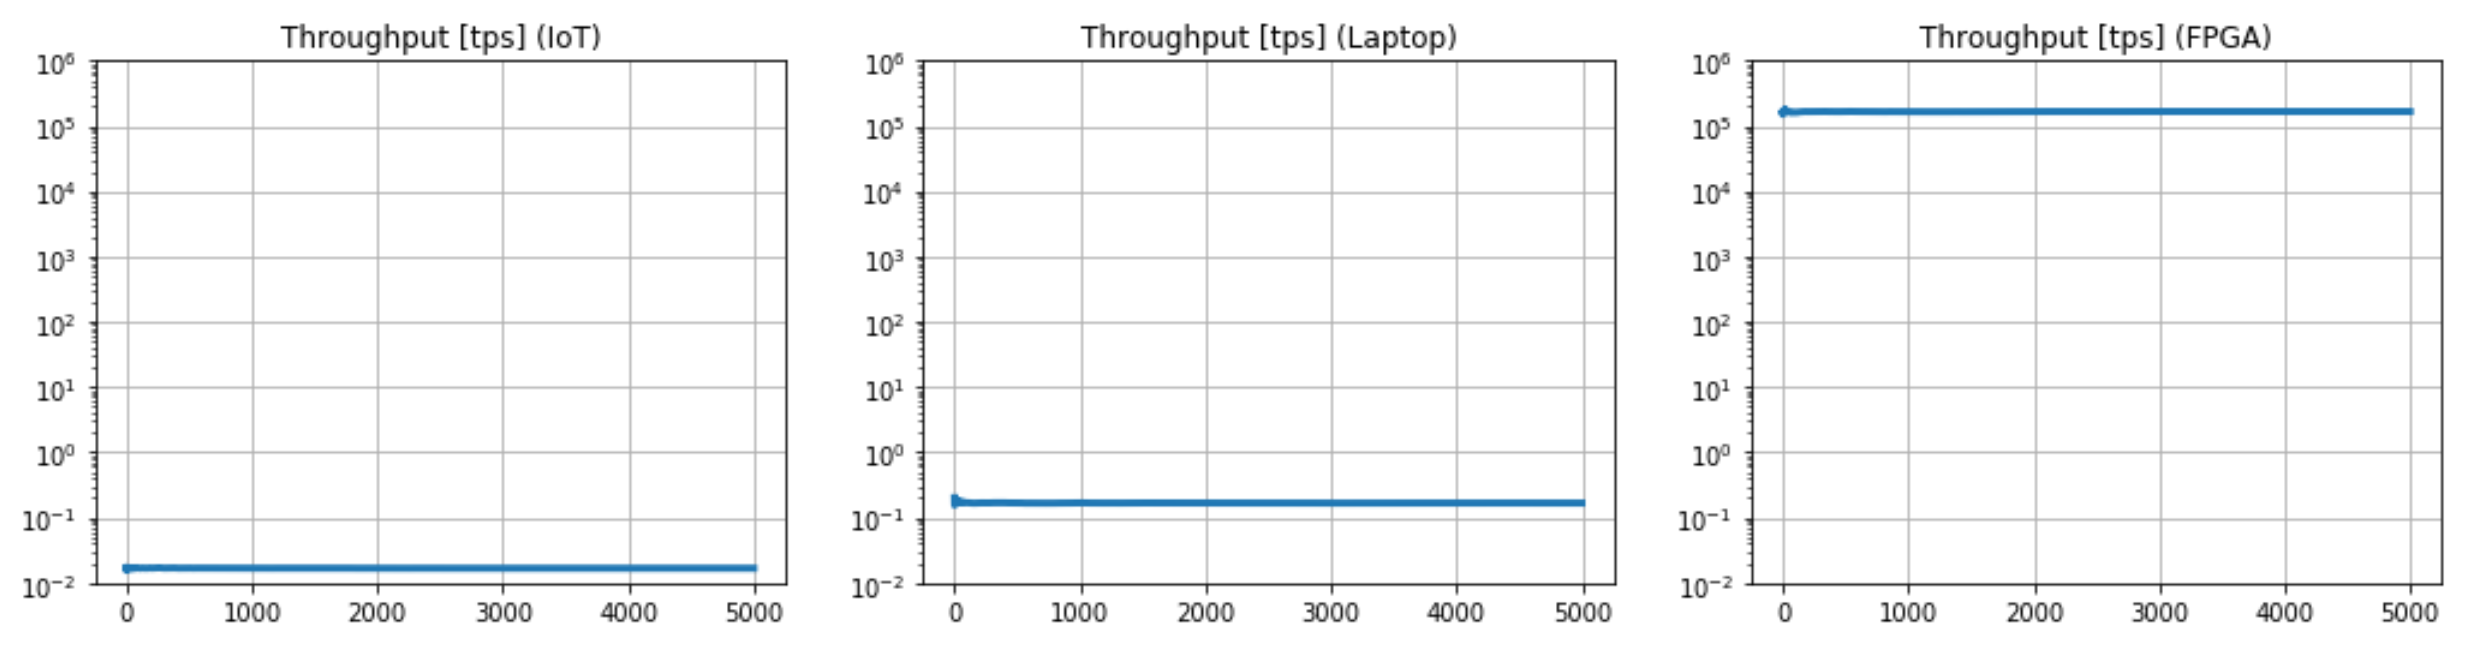
\includegraphics[width=\linewidth]{images/tps_fixed.PNG}
        \caption{Throughput (in transactions per second) with fixed PoW (difficulty = 14).}
        \label{fig:tps_fixed}
    \end{subfigure}
    \caption{Fixed PoW}\label{fig:fixed}
\end{figure*}

In this section, we analyze the adaptive PoW algorithm. In Fig.~\ref{fig:dif_adaptive} we show how the PoW difficulty changes over time. In particular, we see an initial transient phase where the difficulty progressively increases. Then, the difficulty oscillates around a certain value, which depends on the computational capabilities of the device: for instance, IoT devices are able to solve a PoW with difficulty 14, while FPGAs can solve up to a difficulty of 27.

Such a different difficulty mitigates the gap between the solution time for the PoW between the different devices: while IoT can solve the puzzle faster than in the fixed scenario, high power devices see their PoW time raising considerably. This is the key principle behind the adaptive PoW algorithm: make life easy to IoT devices (which is one of the most important IOTA use cases), while bound the power of FPGAs and ASICs (Fig.~\ref{fig:time_adaptive}).

In fact, it is interesting to see that specialized hardware cannot spam the network indefinitely or create congestion, because its allowed throughput is capped in the same order of magnitude of low-power devices. Fig.~\ref{fig:tps_adaptive} shows this fundamental result, which proves the validity of the proposed approach.

\begin{figure*}
    \centering
    \begin{subfigure}[b]{\textwidth}
        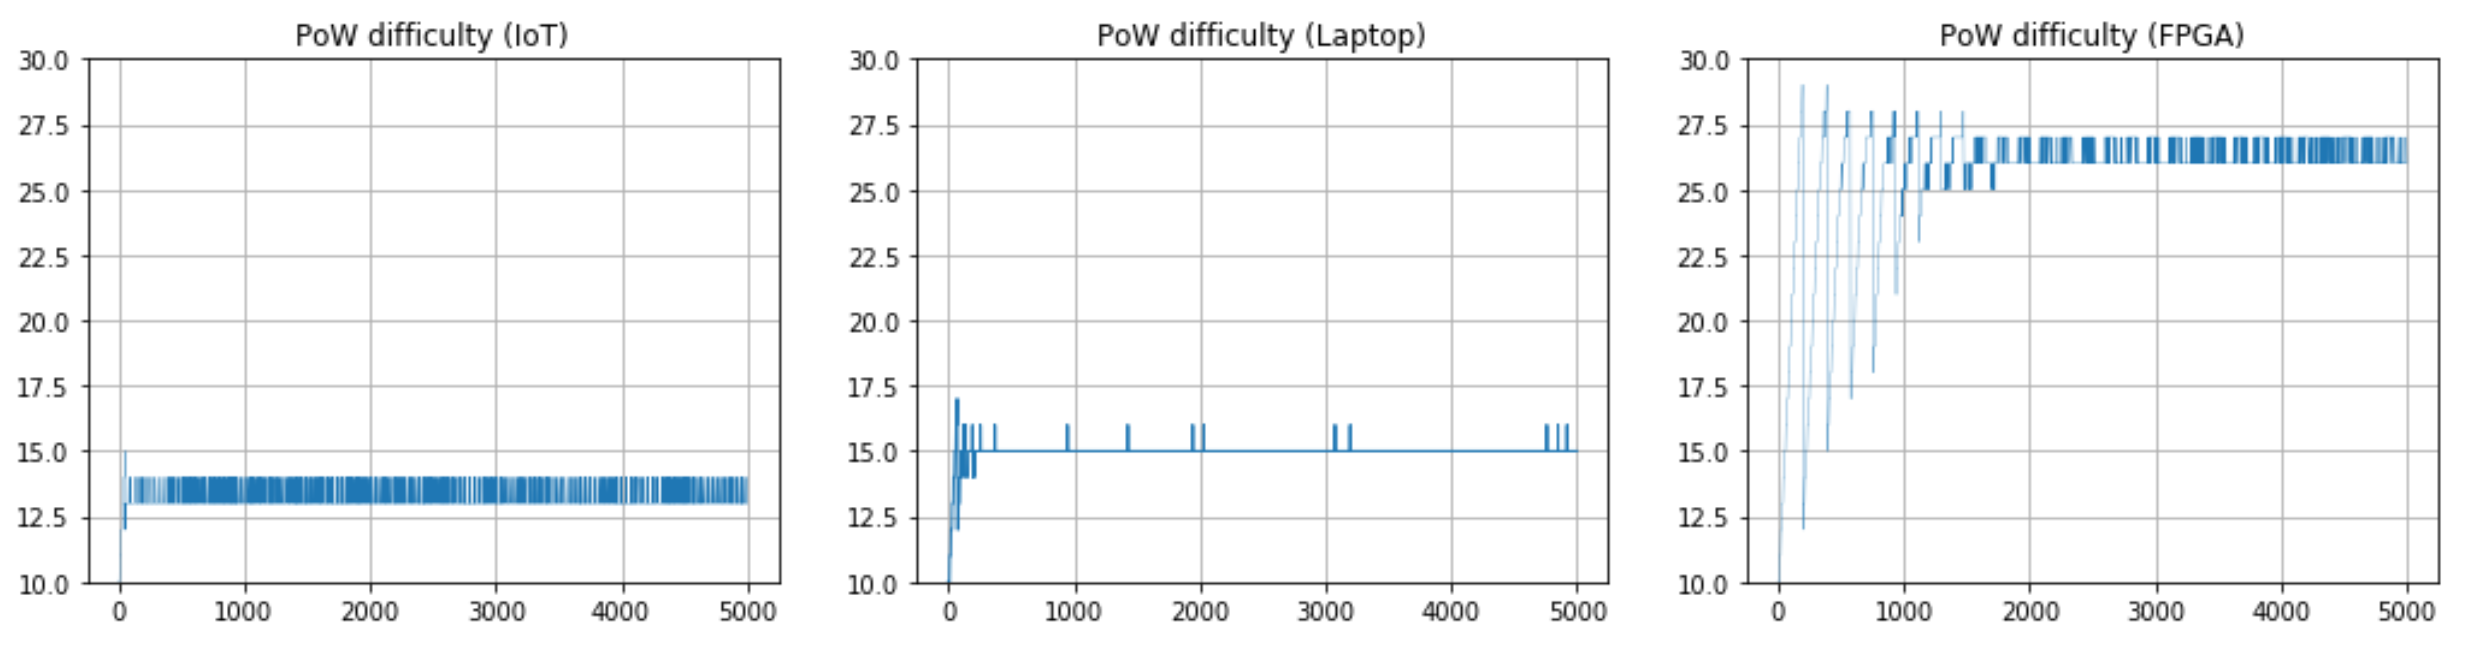
\includegraphics[width=\linewidth]{images/dif_adaptive.PNG}
        \caption{PoW difficulty variation over time.}
        \label{fig:dif_adaptive}
    \end{subfigure}
    
    \begin{subfigure}[b]{\textwidth}
        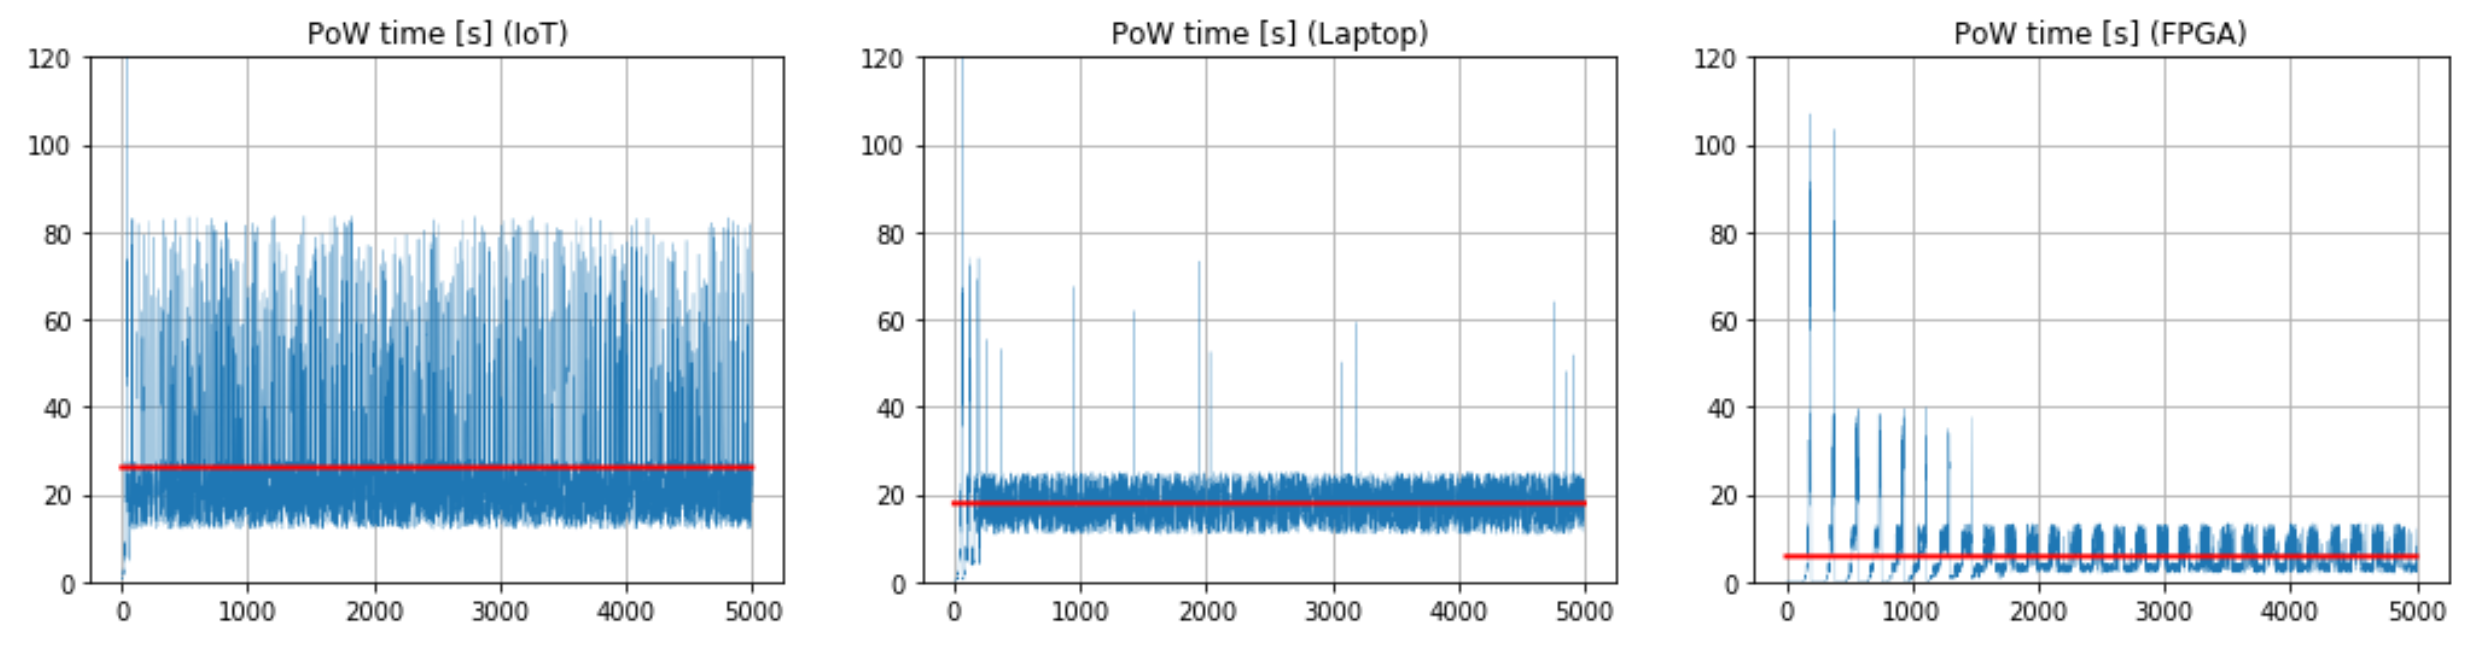
\includegraphics[width=\linewidth]{images/time_adaptive.PNG}
        \caption{Time (in seconds) needed to compute adaptive PoW. The red line shows the average PoW time.}
        \label{fig:time_adaptive}
    \end{subfigure}
    
    \begin{subfigure}[b]{\textwidth}
        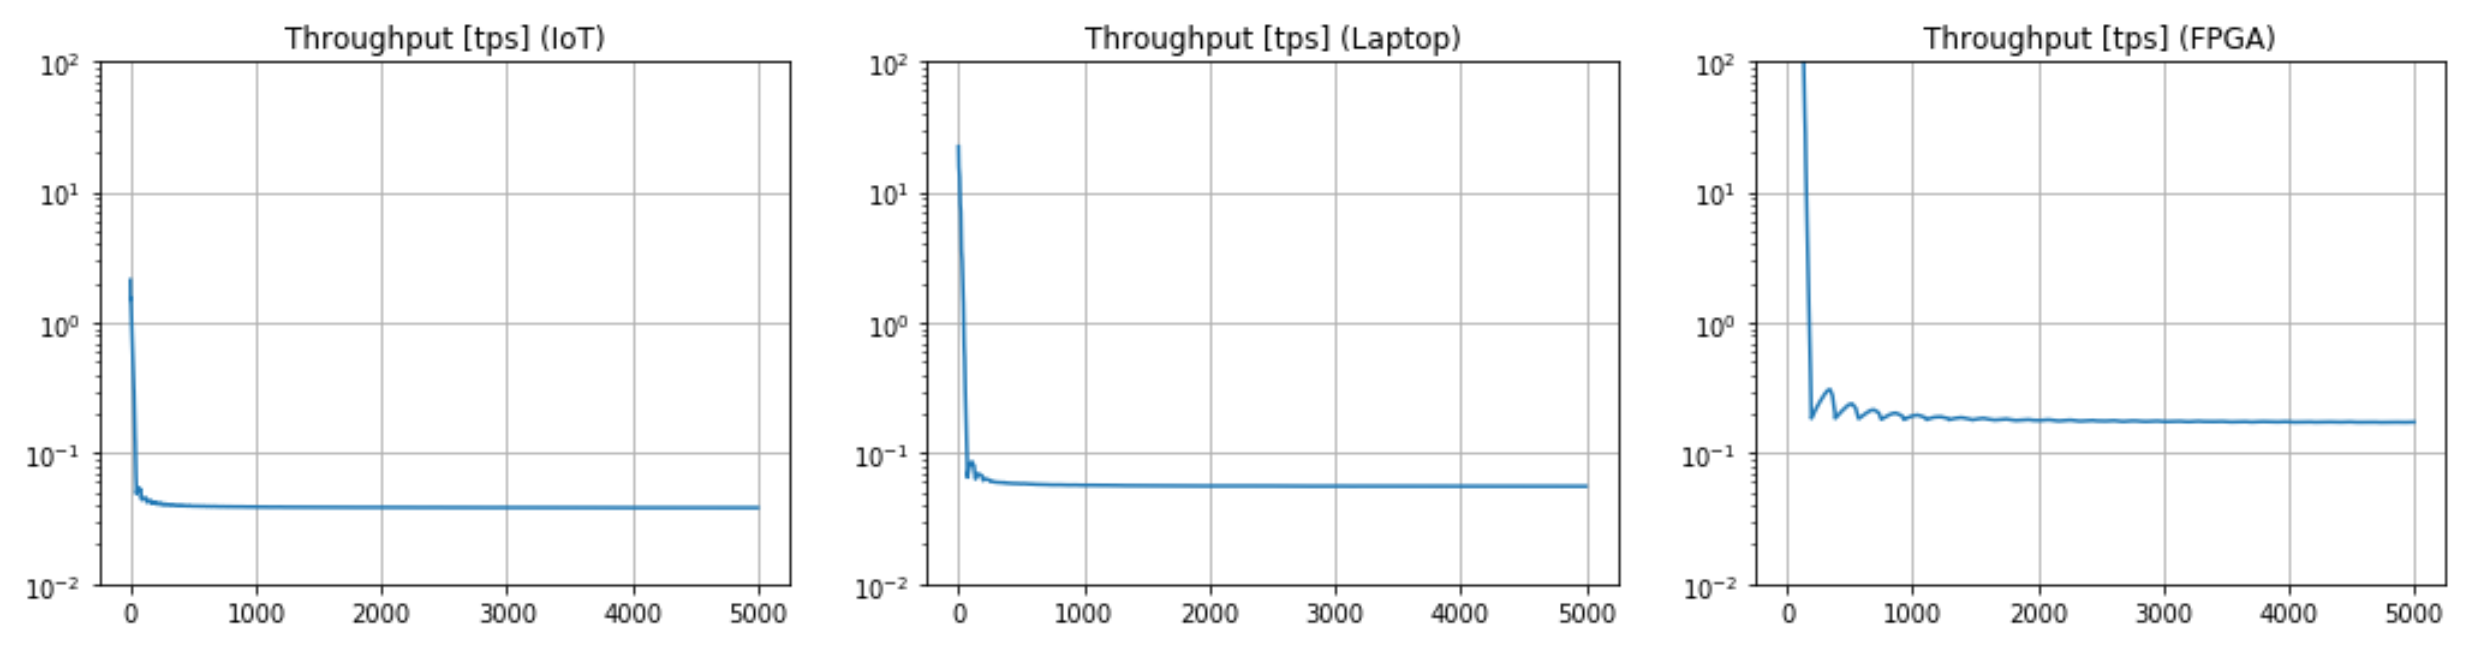
\includegraphics[width=\linewidth]{images/tps_adaptive.PNG}
        \caption{Throughput (in transactions per second) with adaptive PoW.}
        \label{fig:tps_adaptive}
    \end{subfigure}
    \caption{Adaptive PoW}\label{fig:adaptive}
\end{figure*}

\end{document}
